\chapter{Consistency of the MLE -- Wald's Theorem}

\subsubsection*{Setup}

\begin{itemize}
  \item \textbf{Model:}
  \(
    \mathcal{P} = \{\mathsf{P}_{\theta} : \theta \in \Theta\}, \qquad \Theta \subseteq \mathbb{R}^d .
  \)

  \item \textbf{Data:}
  $X_1,\dots,X_n$ i.i.d.\ from $\mathsf{P}_{\theta_0}$, where $\theta_0 \in \Theta$ denotes the \textbf{true parameter} and the sample space is $\mathcal{X}$.

  \item \textbf{Maximum likelihood estimator (MLE):}
  \[
    \hat{\theta}_n
    =
    \arg\max_{\theta \in \Theta} \ell_n(\theta)
    =
    \arg\max_{\theta \in \Theta} \frac{1}{n}\bigl[\ell_n(\theta)-\ell_n(\theta_0)\bigr].
  \]
\end{itemize}

\subsubsection{Asymptotic log-likelihood and Kullback--Leibler divergence}

For every $\theta \in \Theta$,
\begin{equation*}
\label{eq:lln-kl}
\begin{aligned}
\frac{1}{n}\bigl[\ell_n(\theta)-\ell_n(\theta_0)\bigr]
&=
\frac{1}{n}\sum_{i=1}^n
\log\frac{p_\theta(X_i)}{p_{\theta_0}(X_i)}
\\
&\xrightarrow{\text{a.s.}}
\mathsf{E}_{\theta_0}\!\left[
\log\frac{p_\theta(X_1)}{p_{\theta_0}(X_1)}
\right]
=
-\,\mathrm{KL}(\mathsf{P}_{\theta_0}\mid\mathsf{P}_{\theta}).
\end{aligned}
\end{equation*}

Moreover,
\[
\theta_0
=
\arg\max_{\theta \in \Theta}
\bigl\{-\mathrm{KL}(\mathsf{P}_{\theta_0}\mid\mathsf{P}_{\theta})\bigr\},
\]
and the maximizer is unique under identifiability assumptions (A0).

\medskip

\begin{question}
Under which conditions does
\(
\hat{\theta}_n \xrightarrow{\text{a.s.}} \theta_0
\)
hold?
\end{question}

\subsubsection{Why pointwise convergence is not enough}

\begin{ex}[Deterministic counterexample]
Let $\theta \in [0,1]$ and define
\[
f_n(\theta)
=
\sqrt{2\mathrm{e}n}\,\theta(1-\theta^2)^n
-
\Bigl(\theta-\tfrac12\Bigr)^2.
\]
Then
\[
f_n(\theta) \longrightarrow
f(\theta) = -\Bigl(\theta-\tfrac12\Bigr)^2
\quad\text{pointwise as } n\to\infty.
\]
However,
\[
\arg\max_{\theta \in [0,1]} f_n(\theta) \longrightarrow 0
\neq
\tfrac12
=
\arg\max_{\theta \in [0,1]} f(\theta).
\]
as \(n \to \infty\). E.g., note that 
\[
    \lim\limits_{n \to \infty} f_{n}\left(\frac{1}{\sqrt{2n} }\right) = \frac{3}{4} >0.
\]

\end{ex}

\begin{figure}[htpb]
    \centering
    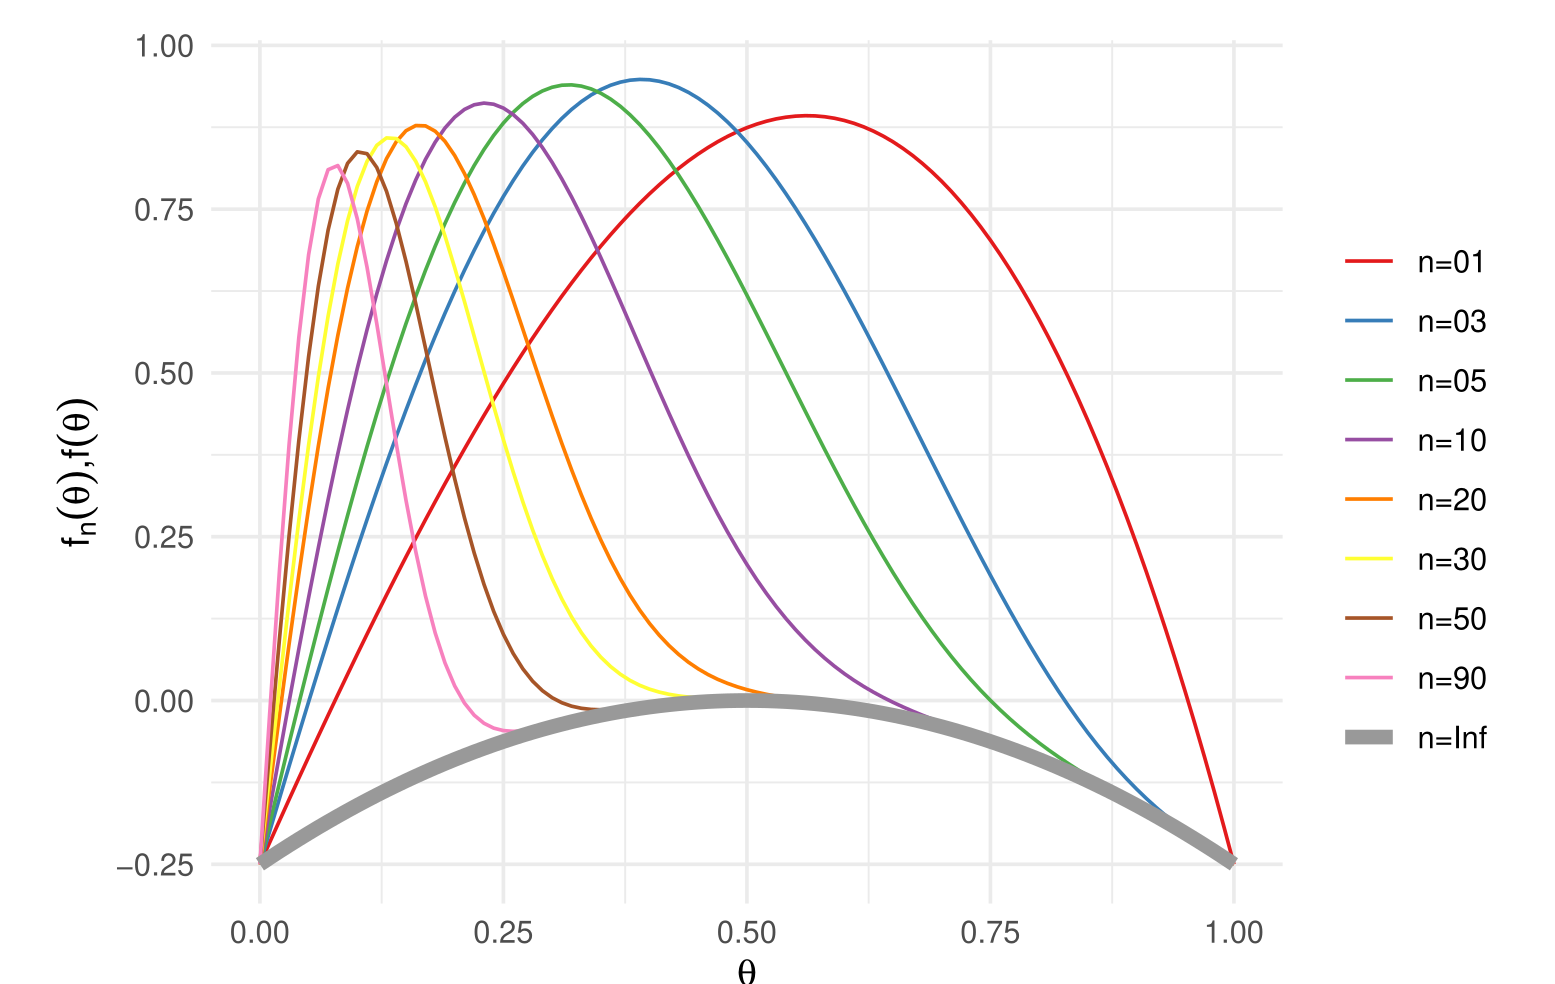
\includegraphics[width=0.8\textwidth]{img/converge}
    \caption{}
    \label{fig:img-converge}
\end{figure}

\begin{remark}
Pointwise convergence of objective functions does \emph{not} guarantee convergence of maximizers.
Some form of \textbf{uniform control} is required to prevent the maximizer from ``escaping''.
\end{remark}

\section{Achieving the Maximum}

%\subsection{Upper Semi-Continuity and Compactness}

\begin{definition}[Upper semi-continuity]
A function $g:\Theta \to \mathbb{R}$ is called \textbf{upper semi-continuous} (u.s.c.) at $\theta_0 \in \Theta$ if
\begin{equation*}
\theta_n \to \theta_0 \quad \Longrightarrow \quad \limsup_{n \to \infty} g(\theta_n) \le g(\theta_0).
\end{equation*}
The function $g$ is called upper semi-continuous if it is u.s.c.\ at every point of its domain.
\end{definition}

\begin{lemma}[Existence of a maximizer on compact sets]
\label{lem:usc-compact-max}
If $g:\Theta \to \mathbb{R}$ is upper semi-continuous, then $g$ achieves its maximum on any compact subset $\Theta_0 \subseteq \Theta$.
\end{lemma}

\begin{proof}
Let
\begin{equation*}
g^* = \sup_{\theta \in \Theta_0} g(\theta).
\end{equation*}
There exists a sequence $(\theta_n)_{n \ge 1} \subset \Theta_0$ such that $g(\theta_n) \to g^*$. Since $\Theta_0$ is compact, there exists a convergent subsequence $(\theta_{n_k})_{k \ge 1}$ with limit $\theta^* \in \Theta_0$. By upper semi-continuity,
\begin{equation*}
g^* = \lim_{k \to \infty} g(\theta_{n_k})
\le g(\theta^*)
\le \sup_{\theta \in \Theta_0} g(\theta)
= g^*.
\end{equation*}
Hence, $g(\theta^*) = g^*$ and the maximum is achieved.
\end{proof}

\bigskip

%\subsection{Motivation from Maximum Likelihood Estimation}

\begin{note}
In the context of maximum likelihood estimation, the function $g$ will typically be the normalized log-likelihood
\[
g_n(\theta) = \frac{1}{n}\ell_n(\theta),
\]
or a log-likelihood ratio. Compactness of the parameter space $\Theta$ and upper semi-continuity of $g_n$ ensure the existence of maximizers for each sample size $n$.
\end{note}

\begin{remark}
Pointwise convergence of $g_n(\theta)$ to a limiting function $g(\theta)$ does \emph{not} in general imply convergence of the maximizers. Additional uniformity conditions are required to prevent the maximizers from ``escaping''.
\end{remark}

\subsubsection{Failure of Pointwise Convergence}

\begin{ex}[Deterministic counterexample]
Consider the sequence of functions $f_n:[0,1]\to\mathbb{R}$ defined by
\begin{equation*}
f_n(\theta)
=
\sqrt{2 e n}\,\theta(1-\theta^2)^n
-
\left(\theta - \tfrac{1}{2}\right)^2.
\end{equation*}
Then $f_n(\theta) \to f(\theta) = -(\theta - \tfrac{1}{2})^2$ pointwise as $n \to \infty$. The limit function has a unique maximizer at $\theta = \tfrac{1}{2}$.
However,
\begin{equation*}
\arg\max_{\theta \in [0,1]} f_n(\theta) \longrightarrow 0
\quad \text{as } n \to \infty,
\end{equation*}
and thus the maximizers do not converge to the maximizer of the limiting function.
\end{ex}

\begin{remark}
This example illustrates the need for uniform control over the log-likelihood surface. In maximum likelihood theory, this role is played by assumptions ensuring that likelihoods cannot take excessively large values away from the true parameter.
\end{remark}

\section{One-Sided Version of a Uniform Law of Large Numbers}

We apply the following result to the special case
\begin{equation*}
f(x,\theta) := \log p_{\theta}(x) - \log p_{\theta_0}(x).
\end{equation*}

\begin{theo}[One-sided uniform law of large numbers]
\label{theo:one-sided-ulln}
Suppose that:
\begin{enumerate}[label=\alph*)]
	\item $\Theta$ is compact;
	\item for all $x \in \mathcal{X}$, the map
	\begin{equation*}
	\theta \mapsto f(x,\theta) := \log p_{\theta}(x) - \log p_{\theta_0}(x)
	\end{equation*}
	is upper semi-continuous;
	\item there exists a measurable function $F:\mathcal{X}\to\mathbb{R}$ such that
	\begin{equation*}
	f(x,\theta) \le F(x)
	\quad \forall x\in\mathcal{X},\ \forall \theta\in\Theta,
	\qquad
	\mathsf{E}_{\theta_0}[F(X)] < \infty;
	\end{equation*}
	\item for all $\theta \in \Theta$ and all sufficiently small $\rho>0$, the function
	\begin{equation*}
	\psi(x,\theta,\rho)
	:=
	\sup_{\|\theta'-\theta\|<\rho} f(x,\theta')
	\end{equation*}
	is measurable in $x$.
\end{enumerate}
Then
\begin{equation*}
\limsup_{n\to\infty}
\sup_{\theta\in\Theta}
\frac{1}{n}\sum_{i=1}^n f(X_i,\theta)
\stackrel{a.s.}{\le}
\sup_{\theta\in\Theta}
\mathsf{E}_{\theta_0}[f(X_1,\theta)].
\end{equation*}
\end{theo}

\begin{remark}
In maximum likelihood applications, $f$ is the log density ratio comparing $p_\theta$ to the true density $p_{\theta_0}$. The theorem ensures that, even after taking a supremum over a continuum of parameter values, the empirical log-likelihood cannot asymptotically exceed the supremum of its population counterpart.
\end{remark}

\begin{proof}[]
The argument follows the spirit of the Glivenko--Cantelli theorem:
\begin{enumerate}[label=\roman*)]
	\item Control expectations of suprema over sufficiently small neighborhoods;
	\item Cover the compact parameter space by finitely many such neighborhoods.
\end{enumerate}

In detail,
\begin{enumerate}[label=\roman*.]
\item
Fix $\theta\in\Theta$. As $\rho\searrow 0$, upper semi-continuity implies
\begin{equation*}
\psi(x,\theta,\rho) \searrow f(x,\theta)
\qquad \text{for all } x\in\mathcal{X}.
\end{equation*}
Indeed, the supremum is attained on the closed ball, and the values of the maximizing sequence converge to the value at the center by upper semi-continuity.

Consequently,
\begin{equation*}
0 \le F(x)-\psi(x,\theta,\rho) \nearrow F(x)-f(x,\theta),
\end{equation*}
and by the monotone convergence theorem,
\begin{equation*}
\mathsf{E}_{\theta_0}[F(X_1)-\psi(X_1,\theta,\rho)]
\longrightarrow
\mathsf{E}_{\theta_0}[F(X_1)-f(X_1,\theta)]
\quad \text{as } \rho\to 0.
\end{equation*}
Since $\mathsf{E}_{\theta_0}[F(X_1)]<\infty$, this yields
\begin{equation*}
\mathsf{E}_{\theta_0}[\psi(X_1,\theta,\rho)]
\longrightarrow
\mathsf{E}_{\theta_0}[f(X_1,\theta)]
=: g(\theta).
\end{equation*}
Hence, for all $\varepsilon>0$ and all $\theta\in\Theta$, there exists $\rho_\theta>0$ such that
\begin{equation*}
\mathsf{E}_{\theta_0}[\psi(X_1,\theta,\rho_\theta)]
<
g(\theta)+\varepsilon.
\end{equation*}

\item
Define the open balls
\begin{equation*}
S(\theta,\rho)
:=
\{\theta'\in\Theta:\|\theta'-\theta\|<\rho\}.
\end{equation*}
Then
\begin{equation*}
\Theta \subseteq \bigcup_{\theta\in\Theta} S(\theta,\rho_\theta).
\end{equation*}
By compactness, there exist $\theta_1,\dots,\theta_m\in\Theta$ such that
\begin{equation*}
\Theta \subseteq \bigcup_{j=1}^m S(\theta_j,\rho_{\theta_j}).
\end{equation*}
Therefore,
\begin{equation*}
\begin{aligned}
\sup_{\theta\in\Theta}\frac{1}{n}\sum_{i=1}^n f(X_i,\theta)
&\le
\sup_{1\le j\le m}
\frac{1}{n}\sum_{i=1}^n
\psi(X_i,\theta_j,\rho_{\theta_j}) \\
&\xrightarrow{a.s.}
\sup_{1\le j\le m}
\mathsf{E}_{\theta_0}[\psi(X_1,\theta_j,\rho_{\theta_j})] \\
&\le
\sup_{1\le j\le m} g(\theta_j) + \varepsilon
\le
\sup_{\theta\in\Theta} g(\theta) + \varepsilon.
\end{aligned}
\end{equation*}
Since $\varepsilon>0$ is arbitrary, the claim follows.
\end{enumerate}
\end{proof}

%\subsection{Upper Semi-Continuity of the Limiting Criterion}

\begin{lemma}
\label{lem:usc}
Under the assumptions of \autoref{theo:one-sided-ulln}, the function
\begin{equation*}
g(\theta)
=
\mathsf{E}_{\theta_0}[f(X_1,\theta)]
\end{equation*}
is upper semi-continuous on $\Theta$.
\end{lemma}

\begin{proof}
Let $\theta_n\to\theta$. By Fatou--Lebesgue,
\begin{equation*}
\begin{aligned}
\limsup_{n\to\infty} g(\theta_n)
&=
\limsup_{n\to\infty} \mathsf{E}_{\theta_0}[f(X_1,\theta_n)] \\
&\le
\mathsf{E}_{\theta_0}\!\left[\limsup_{n\to\infty} f(X_1,\theta_n)\right]
\le
\mathsf{E}_{\theta_0}[f(X_1,\theta)]
=
g(\theta),
\end{aligned}
\end{equation*}
where the last inequality uses upper semi-continuity of $f(x,\cdot)$ for every $x$.
\end{proof}

\subsubsection{Application to Maximum Likelihood}

\begin{remark}
In the likelihood setting,
\begin{equation*}
g(\theta)
=
\mathsf{E}_{\theta_0}\!\left[
\log\frac{p_\theta(X_1)}{p_{\theta_0}(X_1)}
\right]
=
-\,\mathrm{KL}(\mathsf{P}_{\theta_0}\,||\,\mathsf{P}_{\theta}).
\end{equation*}
Thus, upper semi-continuity of the log density ratio implies upper semi-continuity of the negative Kullback--Leibler divergence.
\end{remark}

\begin{note}
The combination of compactness, upper semi-continuity, and the one-sided uniform law of large numbers forms the technical backbone of Wald's consistency theorem for maximum likelihood estimators.
\end{note}


\section{Wald's Theorem}

We study conditions under which maximum likelihood estimators (MLEs) converge to the true parameter. The key technical ingredient is a uniform (one-sided) law of large numbers that prevents the likelihood from ``escaping'' to large values away from the truth.

\begin{definition}[Log density ratio]
Let $\{p_\theta:\theta\in\Theta\}$ be a parametric family of densities and let $\theta_0$ denote the true parameter. Define
\begin{equation*}
f(x,\theta) := \log p_\theta(x) - \log p_{\theta_0}(x).
\end{equation*}
\end{definition}

\begin{definition}[Identifiability]
\label{def:identifiability}
The model is said to be identifiable if
\begin{equation*}
\mathsf{P}_\theta = \mathsf{P}_{\theta_0} \implies \theta = \theta_0.
\end{equation*}
\end{definition}

\begin{theo}[Wald's Theorem 1949]
\label{theo:wald}
Suppose that:
\begin{enumerate}[label=(\alph*)]
	\item $\Theta$ is compact;
	\item $\forall x\in\mathcal{X}$, the map $\theta\mapsto p_\theta(x)$ is upper semi-continuous;
	\item there exists a measurable function $F:\mathcal{X}\to\mathbb{R}$ such that
	\begin{equation*}
	f(x,\theta) \le F(x)
	\quad \forall x\in\mathcal{X},\ \forall \theta\in\Theta,
	\qquad
	\mathsf{E}_{\theta_0}[F(X_1)] < \infty;
	\end{equation*}
	\item for all $\theta\in\Theta$ and all sufficiently small $\rho>0$, the function
	\begin{equation*}
	x\mapsto \sup_{\|\theta'-\theta\|<\rho} f(x,\theta')
	\end{equation*}
	is measurable;
	\item the identifiability condition of \autoref{def:identifiability} holds.
\end{enumerate}
Then any sequence of (possibly non-measurable) maximum likelihood estimators $\hat{\theta}_n$ satisfies
\begin{equation*}
\hat{\theta}_n \xrightarrow{a.s.} \theta_0.
\end{equation*}
\end{theo}

\begin{remark}
The estimator $\hat{\theta}_n$ need not be measurable. The almost sure convergence statement is interpreted pathwise, that is, as a statement about data sequences outside a null set. Conditions ensuring measurability can be found in Ferguson (1996).
\end{remark}

\subsubsection{Heuristic discussion}

Fix $\theta\in\Theta$. By the law of large numbers,
\begin{equation*}
\frac{1}{n}\sum_{i=1}^n f(X_i,\theta)
\;\xrightarrow{a.s.}\;
\mathsf{E}_{\theta_0}[f(X_1,\theta)]
=
-\,\mathrm{KL}(\mathsf{P}_{\theta_0}\,||\,\mathsf{P}_{\theta}).
\end{equation*}
The limiting criterion is uniquely maximized at $\theta_0$. However, pointwise convergence is not sufficient to ensure convergence of maximizers: without uniform control, maxima may ``run away''. Compactness and integrable domination provide the needed uniformity.

\subsubsection{Uniform control via small balls}

For $\theta\in\Theta$ and $\rho>0$, define
\begin{equation*}
\psi(x,\theta,\rho)
:=
\sup_{\|\theta'-\theta\|<\rho} f(x,\theta').
\end{equation*}

\begin{claim}
If $f(x,\cdot)$ is upper semi-continuous, then for every $x$ and $\theta$,
\begin{equation*}
\psi(x,\theta,\rho) \searrow f(x,\theta)
\quad \text{as } \rho\searrow 0.
\end{equation*}
\end{claim}

\begin{proof}
The supremum is at least $f(x,\theta)$ since $\theta$ belongs to every ball. As $\rho\to0$, any maximizing sequence must converge to $\theta$, and upper semi-continuity implies that the limit cannot exceed $f(x,\theta)$.
\end{proof}

\begin{claim}
\label{cl:expectation-convergence}
For fixed $\theta$,
\begin{equation*}
\mathsf{E}_{\theta_0}[\psi(X_1,\theta,\rho)]
\longrightarrow
\mathsf{E}_{\theta_0}[f(X_1,\theta)]
=: g(\theta)
\quad \text{as } \rho\to0.
\end{equation*}
\end{claim}

\begin{proof}
Since $f(x,\theta)\le F(x)$ for all $\theta$, we have
\begin{equation*}
0 \le F(x)-\psi(x,\theta,\rho) \nearrow F(x)-f(x,\theta).
\end{equation*}
By the monotone convergence theorem and $\mathsf{E}_{\theta_0}[F(X_1)]<\infty$,
\begin{equation*}
\mathsf{E}_{\theta_0}[F(X_1)-\psi(X_1,\theta,\rho)]
\to
\mathsf{E}_{\theta_0}[F(X_1)-f(X_1,\theta)],
\end{equation*}
which implies the claim.
\end{proof}

\begin{note}
For every $\varepsilon>0$ and $\theta\in\Theta$, there exists $\rho_\theta>0$ such that
\begin{equation*}
\mathsf{E}_{\theta_0}[\psi(X_1,\theta,\rho_\theta)]
\le g(\theta)+\varepsilon.
\end{equation*}
\end{note}

\subsubsection{Finite covering argument}

By compactness,
\begin{equation*}
\Theta \subseteq \bigcup_{j=1}^m \{\theta':\|\theta'-\theta_j\|<\rho_{\theta_j}\}.
\end{equation*}
Hence,
\begin{equation*}
\sup_{\theta\in\Theta}\frac{1}{n}\sum_{i=1}^n f(X_i,\theta)
\le
\sup_{1\le j\le m}
\frac{1}{n}\sum_{i=1}^n
\psi(X_i,\theta_j,\rho_{\theta_j}).
\end{equation*}
Each term converges almost surely by the law of large numbers, and the supremum over finitely many indices preserves almost sure convergence.

\begin{proof}[of \autoref{theo:wald}]

Fix $r>0$ and define
\begin{equation*}
S_r := \{\theta\in\Theta:\|\theta-\theta_0\|\ge r\}.
\end{equation*}
Then $S_r$ is compact.

\begin{claim}
\label{cl:Sr}
\begin{equation*}
\mathsf{P}_{\theta_0}\big(\exists N\ \forall n\ge N:\ \hat{\theta}_n\notin S_r\big)=1.
\end{equation*}
\end{claim}

\begin{proof}
Applying the uniform law of large numbers to $S_r$ yields
\begin{equation*}
\limsup_{n\to\infty}\sup_{\theta\in S_r}
\frac{1}{n}\sum_{i=1}^n f(X_i,\theta)
\le
\sup_{\theta\in S_r} g(\theta)
=:\delta
\quad \text{a.s.}
\end{equation*}
By \autoref{lem:usc}, the supremum is attained. Since $\theta_0\notin S_r$ and $g(\theta)<0$ for $\theta\neq\theta_0$, we have $\delta<0$. Hence, eventually
\begin{equation*}
\sup_{\theta\in S_r}\frac{1}{n}\sum_{i=1}^n f(X_i,\theta)
\le \frac{\delta}{2}.
\end{equation*}
On the other hand,
\begin{equation*}
\frac{1}{n}\sum_{i=1}^n f(X_i,\hat{\theta}_n)
=
\sup_{\theta\in\Theta}\frac{1}{n}\sum_{i=1}^n f(X_i,\theta)
\ge 0,
\end{equation*}
which implies $\hat{\theta}_n\notin S_r$ eventually.
\end{proof}

Define
\begin{equation*}
A_r := \{\exists N\ \forall n\ge N:\ \hat{\theta}_n\notin S_r\}.
\end{equation*}
The events $A_r$ are decreasing as $r\searrow0$, and $\mathsf{P}_{\theta_0}(A_r)=1$ for all $r>0$. Therefore,
\begin{equation*}
\mathsf{P}_{\theta_0}\Big(\bigcap_{r>0} A_r\Big)=1,
\end{equation*}
which is exactly the statement $\hat{\theta}_n\to\theta_0$ almost surely.
\end{proof}

\begin{note}
Compactness, upper semi-continuity, and an integrable envelope are indispensable. Without them, global maximizers of the likelihood may fail to be consistent.
\end{note}

\section{Examples for Wald's Theorem}

\begin{ex}[Cauchy location model]
\label{ex:cauchy}

Consider the Cauchy location model with density
\begin{equation*}
p_{\vartheta}(x)
=
\frac{1}{\pi}\frac{1}{1+(x-\vartheta)^2},
\qquad \vartheta\in\mathbb{R}.
\end{equation*}

Since the parameter space $\mathbb{R}$ is not compact, Wald's theorem cannot be applied directly. We therefore reparametrize by
\begin{equation*}
\vartheta = \tan(\theta/2),
\qquad \theta\in(-\pi,\pi),
\end{equation*}
which yields the equivalent family
\begin{equation*}
p_{\theta}(x)
=
\frac{1}{\pi}\frac{1}{1+\bigl(x-\tan(\theta/2)\bigr)^2},
\qquad \theta\in(-\pi,\pi).
\end{equation*}

To compactify the parameter space, define artificial boundary values
\begin{equation*}
p_{\pm\pi}(x)
:=
\lim_{\theta\to\pm\pi} p_\theta(x)
=
\lim_{\vartheta\to\pm\infty} p_\vartheta(x)
=
0,
\qquad \forall x\in\mathbb{R}.
\end{equation*}

This yields a compact parameter space
\begin{equation*}
\Theta = [-\pi,\pi],
\qquad
\mathsf{P} = \{\mathsf{P}_\theta:\theta\in\Theta\}.
\end{equation*}

Without loss of generality, we may take $\theta_0=0$ (otherwise shift the data by $x_i' = x_i-\vartheta_0$).

\subsubsection*{Verification of Wald's conditions}

\begin{enumerate}[label=\alph*)]
\item \textbf{Compactness.}
By construction, $\Theta=[-\pi,\pi]$ is compact.

\item \textbf{Identifiability.}
The median of $\mathsf{P}_\theta$ equals $\tan(\theta/2)$, hence
\begin{equation*}
\theta\neq\theta_0
\;\Longrightarrow\;
\mathsf{P}_\theta\neq\mathsf{P}_{\theta_0},
\qquad \theta_0\in(-\pi,\pi).
\end{equation*}

\item \textbf{Upper semi-continuity.}
For every $x$, the map $\theta\mapsto p_\theta(x)$ is continuous on $(-\pi,\pi)$, and the boundary values were chosen to preserve continuity. Hence $\theta\mapsto p_\theta(x)$ is upper semi-continuous on $\Theta$.

\item \textbf{Measurability.}
Continuity implies measurability. Indeed, for any $A\subseteq\Theta$ and $t\in\mathbb{R}$,
\begin{equation*}
\{x:\sup_{\theta\in A}p_\theta(x)\le t\}
=
\bigcap_{\theta\in A\cap\mathbb{Q}}
\{x:p_\theta(x)\le t\},
\end{equation*}
a countable intersection of measurable sets.

\item \textbf{Integrable envelope.}
The log-likelihood ratio equals
\begin{equation*}
f(x,\theta)
=
\log p_\theta(x)-\log p_{\theta_0}(x)
=
\begin{cases}
\log\!\left(\dfrac{1+x^2}{1+\bigl(x-\tan(\theta/2)\bigr)^2}\right),
& \theta\in(-\pi,\pi),\\[1em]
-\infty,
& \theta=\pm\pi.
\end{cases}
\end{equation*}
Since $1+(x-\tan(\theta/2))^2\ge 1$ for all $\theta$, we have
\begin{equation*}
f(x,\theta)\le \log(1+x^2)=:F(x),
\qquad \forall x,\theta.
\end{equation*}
Moreover,
\begin{equation*}
\mathsf{E}_{\theta_0}[F(X_1)]
=
\int_{\mathbb{R}}
\log(1+x^2)\,
\frac{1}{\pi}\frac{1}{1+x^2}\,\mathrm{d}x
=
2\log 2
<\infty.
\end{equation*}
\end{enumerate}

All assumptions of Wald's theorem are satisfied. Hence the global maximum likelihood estimator in the Cauchy location model is \textbf{consistent}, despite the likelihood exhibiting many local optima.
\end{ex}

\begin{ex}[Normal distribution with unknown mean and variance]
\label{ex:normal}

Consider the normal model
\begin{equation*}
p_{\bs{\theta}}(x)
=
\frac{1}{\sqrt{2\pi\sigma^2}}
\exp\!\left\{-\frac{1}{2\sigma^2}(x-\mu)^2\right\},
\qquad
\bs{\theta}=(\mu,\sigma^2)^{\top}\in\mathbb{R}\times(0,\infty).
\end{equation*}

For i.i.d.\ data $X_1,\dots,X_n\sim\mathsf{P}_{\bs{\theta}_0}$, the MLE is
\begin{equation*}
\hat{\mu}
=
\frac{1}{n}\sum_{i=1}^n X_i,
\qquad
\hat{\sigma}^2
=
\frac{1}{n}\sum_{i=1}^n (X_i-\hat{\mu})^2.
\end{equation*}
By the strong law of large numbers,
\begin{equation*}
\hat{\bs{\theta}}_n
=
(\hat{\mu},\hat{\sigma}^2)^{\top}
\xrightarrow{a.s.}
(\mu_0,\sigma_0^2)^{\top}.
\end{equation*}

\subsubsection*{Why Wald's theorem fails}

Fix $x\in\mathbb{R}$. Maximizing the likelihood over $\theta$ yields
\begin{equation*}
\sup_{\mu,\sigma^2} p_\theta(x)
=
\infty,
\end{equation*}
since setting $\mu=x$ and letting $\sigma^2\to 0$ makes the density diverge. Consequently, the log-likelihood ratio admits no integrable upper bound, and Wald's theorem does not apply.

\subsubsection*{Solution via grouping}

Group observations into pairs
\begin{equation*}
\tilde{X}_1=(X_1,X_2),\;
\tilde{X}_2=(X_3,X_4),\;
\tilde{X}_3=(X_5,X_6),\dots
\end{equation*}
and consider the joint density of $(X_1,X_2)$. One can show that
\begin{equation}
\max_{\theta} p_\theta(x_1,x_2)
=
p_{(\tilde{\mu},\tilde{\sigma}^2)}(x_1,x_2)
=
\frac{2}{e\pi(x_1-x_2)^2},
\label{eq:normal-bound}
\end{equation}
where
\begin{equation*}
\tilde{\mu}=\frac{x_1+x_2}{2},
\qquad
\tilde{\sigma}^2=\frac{1}{4}(x_1-x_2)^2.
\end{equation*}

Since $\mathsf{P}_{\theta_0}(X_1\neq X_2)=1$, the bound in \eqref{eq:normal-bound} is integrable. After compactifying the parameter space as in \autoref{ex:cauchy}, Wald's theorem applies, yielding consistency of the MLE; see van der Vaart (1998, Problem~5.25).
\end{ex}

\begin{remark}
These examples illustrate that Wald's conditions are sufficient but not necessary. The normal MLE is consistent even when Wald's theorem fails in its basic form, while suitable reformulations may restore applicability.
\end{remark}
